\documentclass[8pt]{beamer}
\usepackage{tikz}
\usepackage[utf8]{vietnam}
\usepackage{amsmath}
\usepackage{graphicx}
\usepackage{mathrsfs}
\usepackage{amssymb,amsfonts,amsthm}
\usepackage{wrapfig}
\usepackage{hyperref}
\usetheme{Copenhagen}
\usecolortheme{spruce}
\setbeamertemplate{navigation symbols}{}
\setbeamertemplate{headline}{}
\setbeamertemplate{footline}{}
\title[Kết quả nghiên cứu tuần 1]
{Kết quả nghiên cứu tuần $1$}
\subtitle{Phòng thí nghiệm Thông tin Vô tuyến}
\author[Phòng thí nghiệm thông tin Vô tuyến]
{Tín Vũ}
\date[VLC 2021] % (optional)
{tinvu1309@gmail.com}
\begin{document}
\frame{\titlepage}
\begin{frame}{Mục lục}
\tableofcontents
\end{frame}
\begin{frame}{Tài liệu tham khảo}
\section{Tài liệu tham khảo}
Tài liệu tham khảo được sử dụng để nghiên cứu gồm: Calculus 7E (James Stewart), Antenna Theory (A.Balanis).
\end{frame}
\begin{frame}{Các kết quả cơ bản}
\section{Các kết quả cơ bản}
\begin{itemize}
\item Tích phân đường
\end{itemize}
\subsection{Tích phân đường}
\subsubsection{Tích phân đường vô hướng}
\begin{itemize}
	\item[-] Tích phân đường vô hướng
\end{itemize}
\begin{figure}[h]
			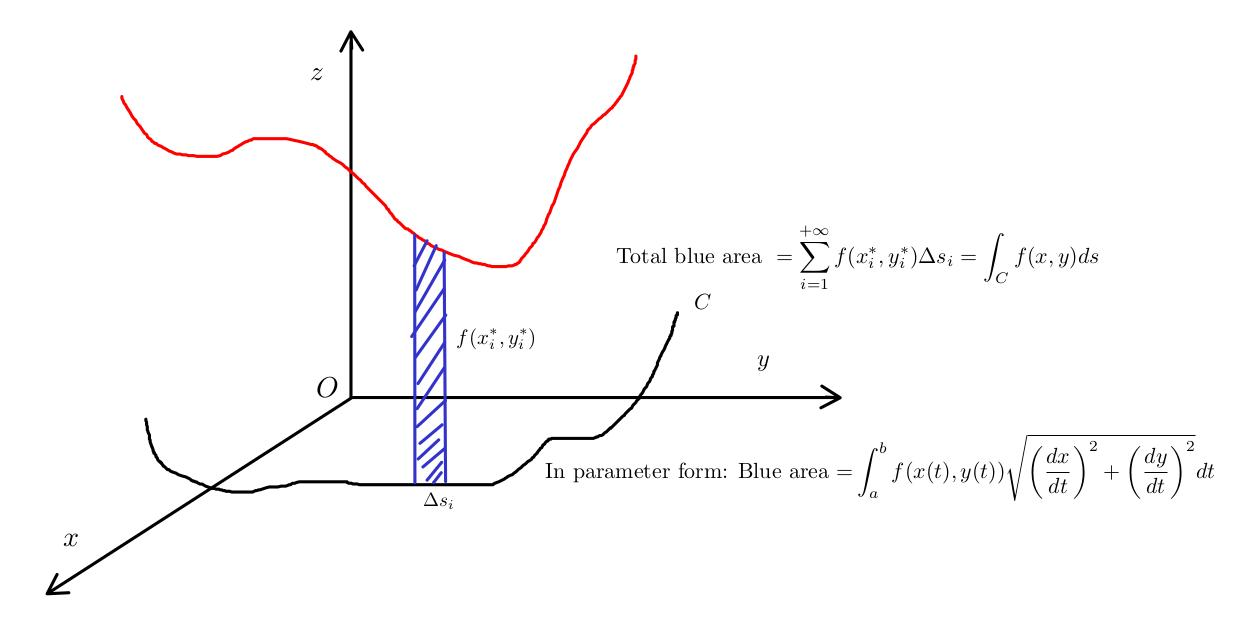
\includegraphics[width=0.9\textwidth]{line.jpg}
			\caption{Scalar line integral}			\label{fig:re1}
\end{figure}
\end{frame}
\begin{frame}{Các kết quả cơ bản}
\begin{itemize}
	\item[-] Tích phân đường có hướng
\end{itemize}
\subsubsection{Tích phân đường có hướng}
\begin{figure}[h]
			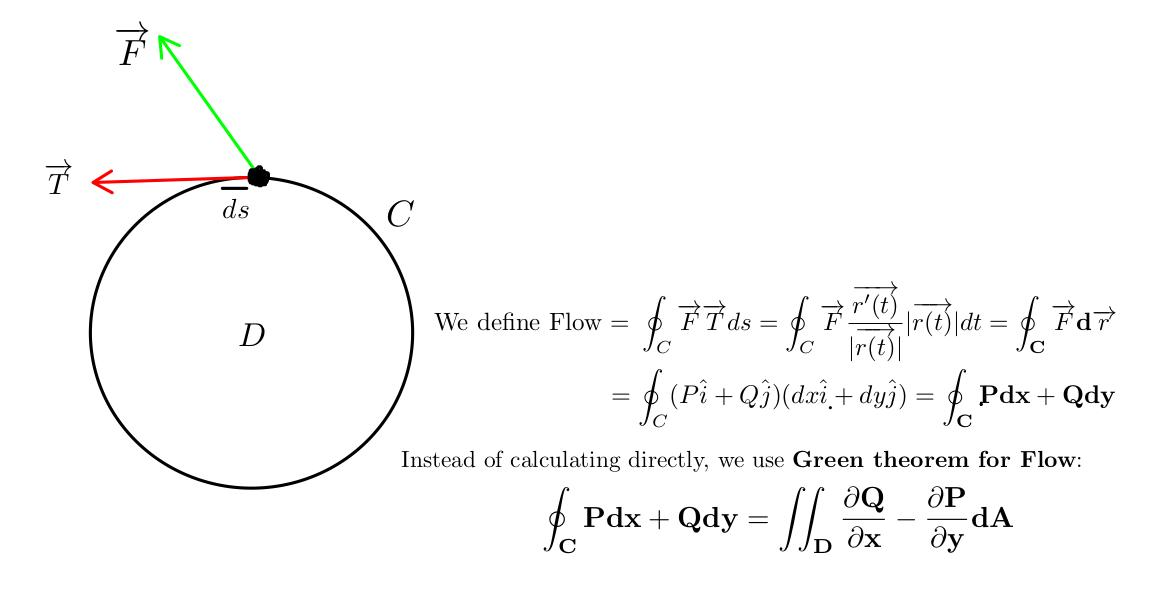
\includegraphics[width=1\textwidth]{green1.jpg}
			\caption{Green's theorem for Flow}			\label{fig:re2}
\end{figure}

\end{frame}
\begin{frame}{Các kết quả cơ bản}
Chúng ta sẽ chứng minh lại định lý Green cho trường hợp đơn giản nhất, xét đường đơn liên kín C như hình vẽ sau:
\begin{figure}[h]
			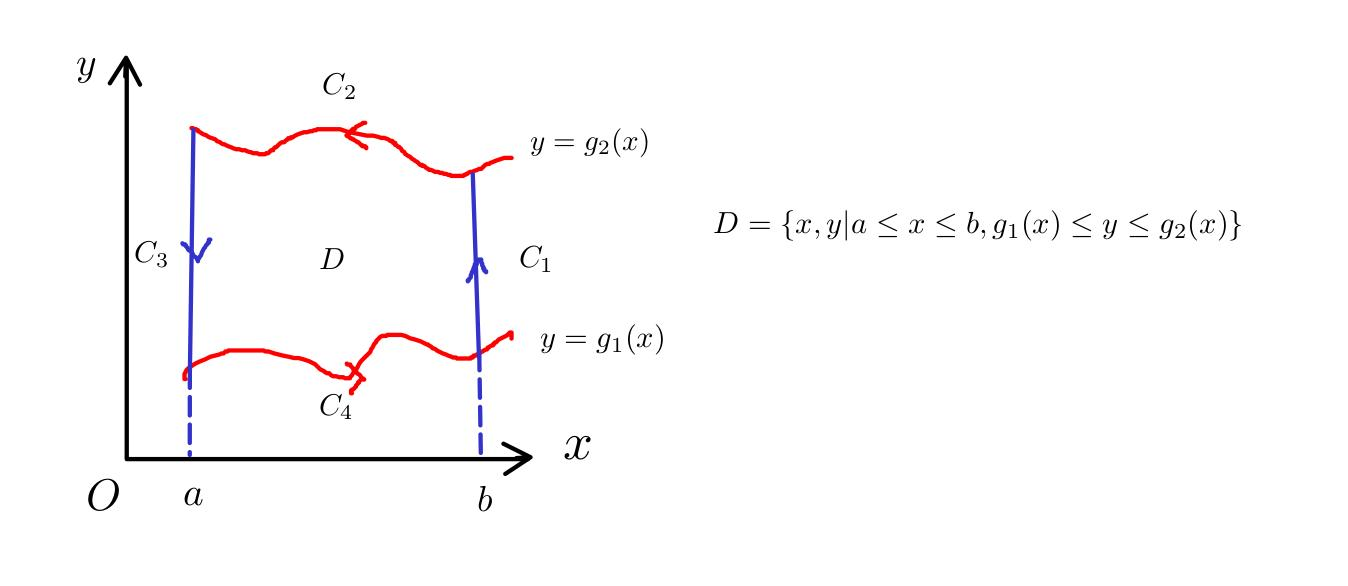
\includegraphics[width=0.9\textwidth]{domain.jpg}
			\caption{Proof of Green's theorem for Flow}			\label{fig:re3}
\end{figure}
Để cho đơn giản, ta chỉ chứng minh đẳng thức: $$\oint_{C}Pdx=-\iint_{D}\frac{\partial P}{\partial y}dA$$
\end{frame}
\begin{frame}{Các kết quả cơ bản}
\begin{equation*}
\begin{split}
	\oint_{C}Pdx &=\int_{a}^{b}P(x,g_{1}(x))+\int_{b}^{a}P(x,g_{2}(x))dx=\int_{a}^{b}P(x,g_{1}(x))dx-\int_{a}^{b}P(x,g_{2}(x))dx\\
	\iint_{D}\frac{\partial P}{\partial y}dA &=\int_{a}^{b}\int_{g_{1}(x)}^{g_{2}(x)}\frac{\partial P}{\partial y}dydx=\int_{a}^{b}P(x,g_{2}(x))dx-\int_{a}^{b}P(x,g_{1}(x))dx\\
						 &\Rightarrow\oint_{C}Pdx=-\iint_{D}\frac{\partial P}{\partial y}dA
\end{split}
\end{equation*}
Chứng minh tương tự, ta cũng thu được $$\oint_{C}Qdy=\iint_{D}\frac{\partial Q}{\partial x}dA\Rightarrow \oint_{C}Pdx+Qdy=\iint_{D}\left(\frac{\partial Q}{\partial x}-\frac{\partial P}{\partial y}\right)dA$$
Ta viết lại công thức Green dạng \textbf{curl}:
$$\oint_{C}Pdx+Qdy=\iint_{D}\textbf{curl}\overrightarrow{F}\hat kdA=\iint_{D}(\nabla \times \overrightarrow{F})\hat kdA$$
\end{frame}
\begin{frame}{Các kết quả cơ bản}
\begin{figure}[h]
			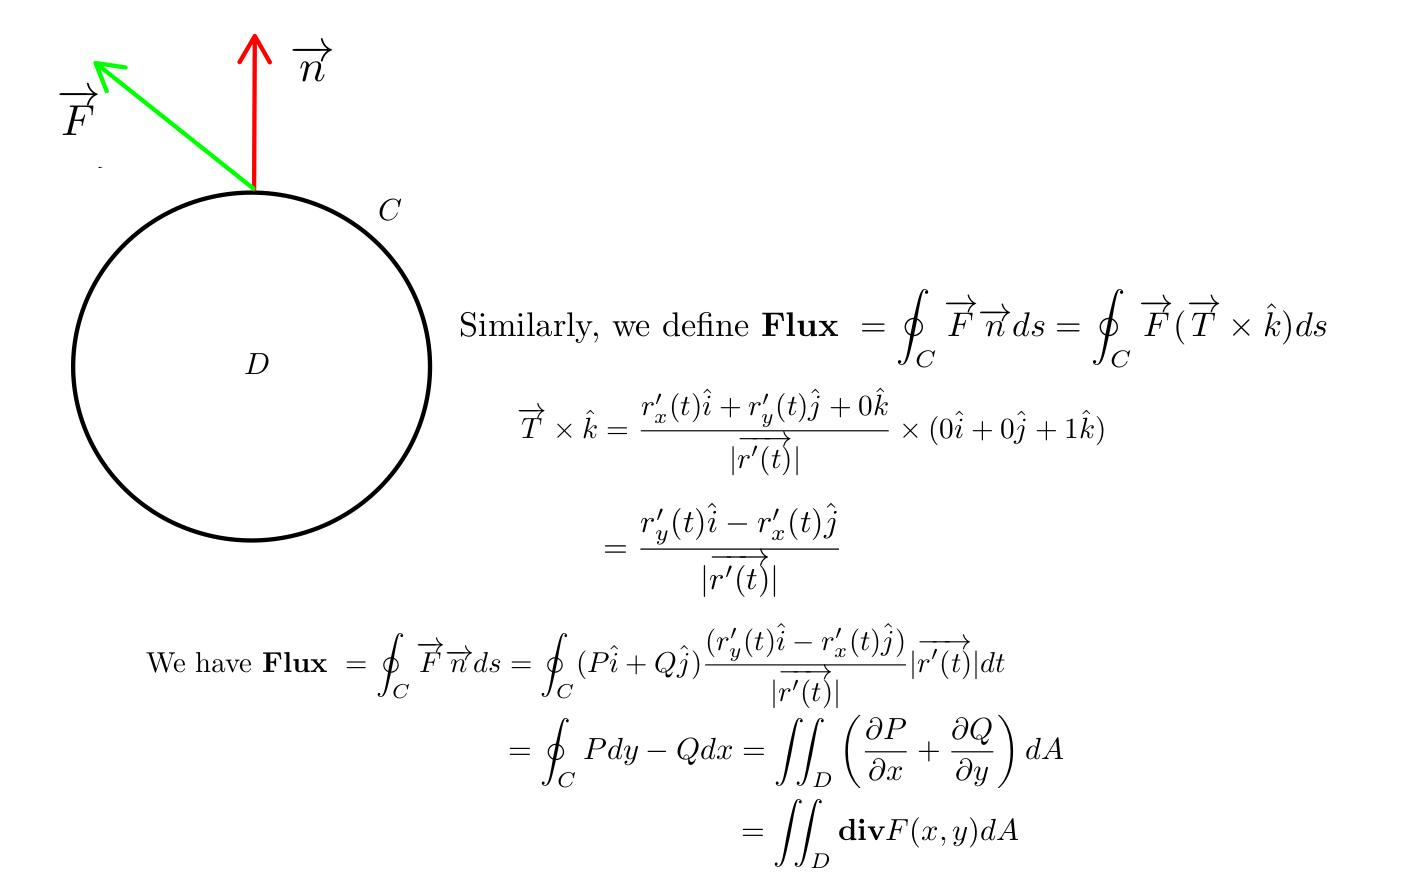
\includegraphics[width=1\textwidth]{flux.jpg}
			\caption{Green's theorem for Flux}			\label{fig:re4}
\end{figure}

\end{frame}
\begin{frame}{Các kết quả cơ bản}
\subsection{Tích phân mặt}
\subsubsection{Diện tích mặt}
\begin{itemize}
	\item Tích phân mặt
\end{itemize}
\begin{itemize}
	\item[-] Diện tích mặt
\end{itemize}
Mọi mặt phẳng bất kì đều có thể được biểu diễn rất dễ dàng qua hàm vector $$\overrightarrow{r(u,v)}=x(u,v)\hat i+y(u,v)\hat j+z(u,v)\hat k$$
Ta xét một mặt bất kì được biểu diễn bởi hàm vector trên, với $(u,v)\in D$, ta muốn tìm diện tích mặt này.
\begin{figure}[h]
			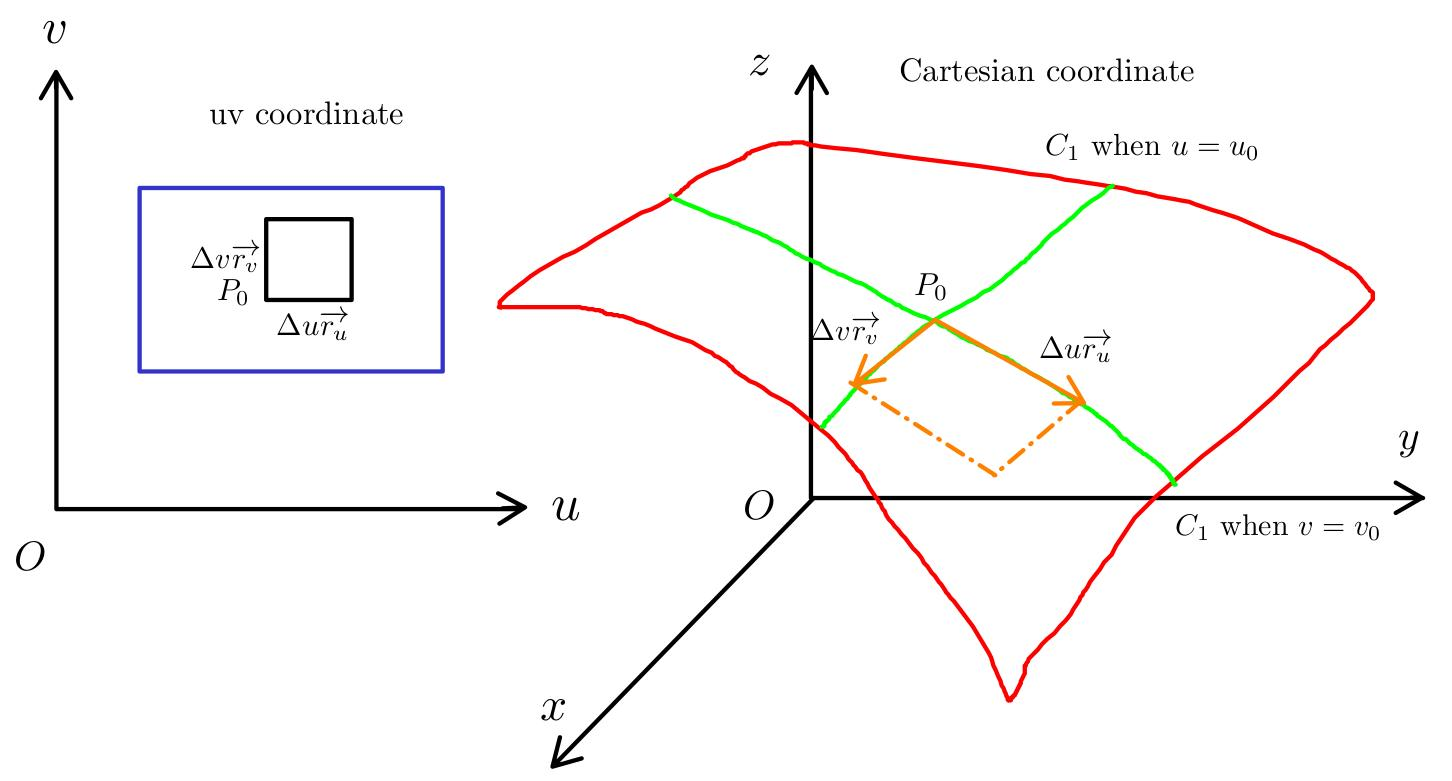
\includegraphics[width=0.8\textwidth]{cartesina.jpg}
			\caption{Surface Area}			\label{fig:re4}
\end{figure}
\end{frame}
\begin{frame}{Các kết quả cơ bản}
	Như đã thảo luận ở slide trước, ta có thể dễ dàng thấy rằng $\overrightarrow{r_{u}}$, $\overrightarrow{r_{v}}$ chính là 2 vector đạo hàm riêng lần lượt của biến $u$ và $v$. Đây chính là cặp vector tiếp tuyến của các đường cong $C_{1}$ và $C_{2}$ (đã chứng minh ở slide trước), với:
\begin{equation*}
\begin{split}
	\overrightarrow{r_{u}}&=\frac{\partial x(u,v)}{\partial u}\hat i+\frac{\partial y(u,v)}{\partial u}\hat j+\frac{\partial z(u,v)}{\partial u}\hat k
\end{split}
\end{equation*}

\begin{equation*}
\begin{split}
	\overrightarrow{r_{v}}&=\frac{\partial x(u,v)}{\partial v}\hat i+\frac{\partial y(u,v)}{\partial v}\hat j+\frac{\partial z(u,v)}{\partial v}\hat k
\end{split}
\end{equation*}
Ta có thể ước lượng xấp xỉ vi phân diện tích một mặt chữ nhật rất nhỏ:
$$dA(S)=|\overrightarrow{(r_{u}}du)\times(\overrightarrow{r_{v}}dv)|=|\overrightarrow{r_{u}}\times\overrightarrow{r_{v}}|dA$$
Vậy ta thu được diện tích toàn bộ mặt phẳng có thể được biểu diễn bằng tổng Riemann trực tiếp, ta viết lại đơn giản hơn như sau:
$$\alert{A(S)=\sum_{i=1}^{m}\sum_{j=1}^{n}|\overrightarrow{r_{u}}\times\overrightarrow{r_{v}}|=\iint_{D}|\overrightarrow{r_{u}}\times\overrightarrow{r_{v}}|dA}$$
Đây là kết quả cực kì quan trọng, sẽ liên tục được sử dụng trong phần tích phân mặt.
\end{frame}
\begin{frame}{Các kết quả cơ bản}
\begin{itemize}
	\item[-] Tích phân mặt vô hướng
\end{itemize}
\subsubsection{Tích phân mặt vô hướng}
\begin{figure}[h]
			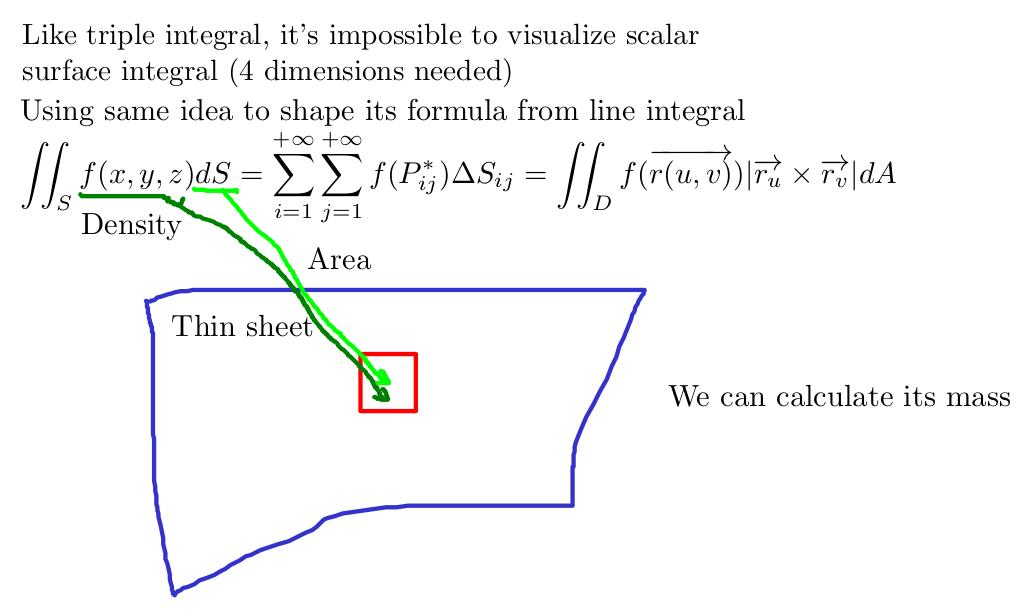
\includegraphics[width=0.9\textwidth]{sheet.jpg}
			\caption{Scalar surface integral}			\label{fig:re5}
\end{figure}

\end{frame}
\begin{frame}{Các kết quả cơ bản}
\subsubsection{Tích phân mặt có hướng}
\begin{itemize}
	\item[-] Tích phân mặt có hướng
\end{itemize}
\begin{figure}[h]
			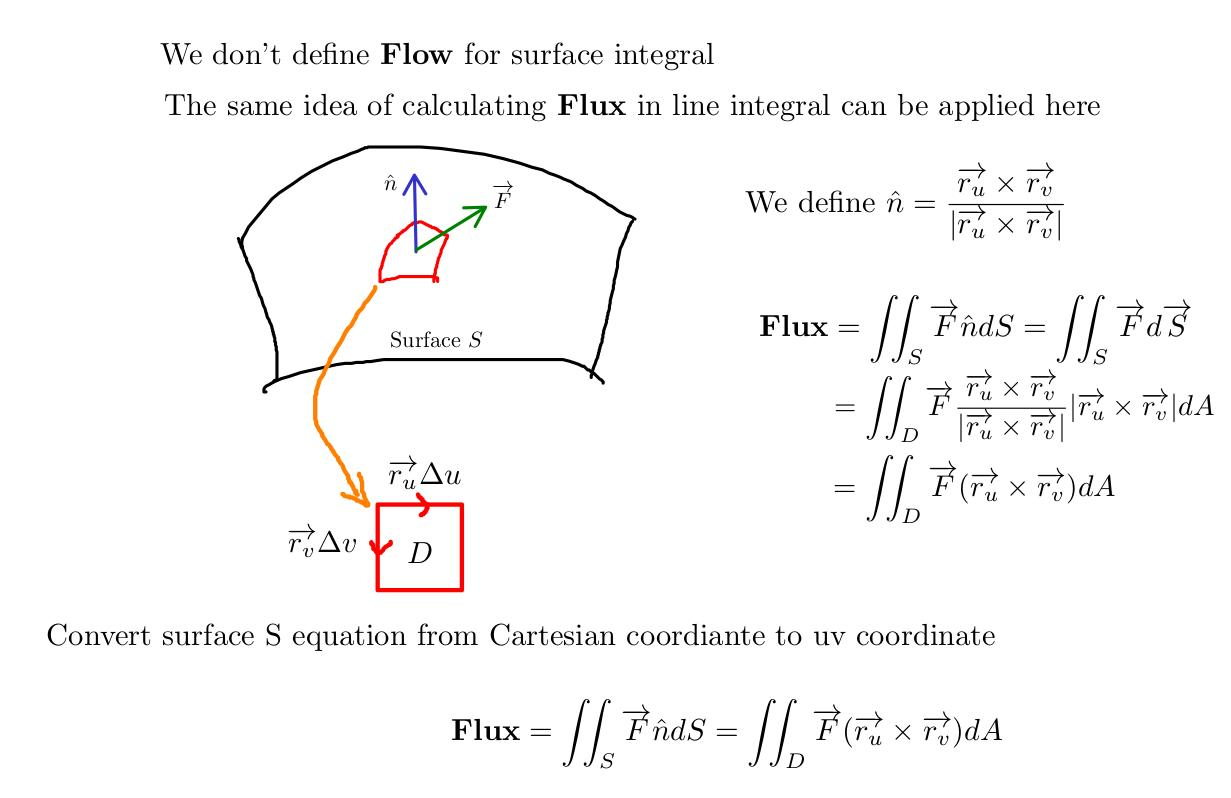
\includegraphics[width=0.9\textwidth]{fluxo.jpg}
			\caption{Flux in surface integral}			\label{fig:re5}
\end{figure}

\end{frame}
\begin{frame}{Các kết quả cơ bản}
Chúng ta tổng quát hóa định lý Green cho \textbf{Flux} và \textbf{Flow} trong không gian 3 chiều:
\begin{block}{Định lý Green trong không gian 2 chiều}
	\begin{equation*}
		\begin{split}
			\textbf{Flux}&=\oint_{C}\overrightarrow{F}\overrightarrow{n}ds=\iint_{D}\textbf{div}\overrightarrow{F}dA=\iint_{D}\nabla\cdot \overrightarrow{F}dA \\
			\textbf{Flow}&=\oint_{C}\overrightarrow{F}\overrightarrow{T}ds=\iint_{D}\textbf{curl}\overrightarrow{F}\hat k dA=\iint_{D}(\nabla\times\overrightarrow{F})\hat k dA
		\end{split}
	\end{equation*}
\end{block}
\begin{block}{Định lý Green trong không gian 3 chiều}
\begin{itemize}
	\item  Định lý phân kỳ (divergence theorem):$$\textbf{Flux}=\iint_{S}\overrightarrow{F}\hat n dS=\iint_{S}\overrightarrow{F}d\overrightarrow{S}=\iiint_{E}\textbf{div}\overrightarrow{F}dV$$
	\item Định lý Stoke: $$\textbf{Flow}=\int_{C}\overrightarrow{F}\overrightarrow{T}dS=\iint_{S}\textbf{curl}\overrightarrow{F}d\overrightarrow{S}$$
\end{itemize}
\end{block}
\end{frame}
\begin{frame}{Lý thuyết Antenna}
\section{Lý thuyết Antenna}
\begin{itemize}
	\item Giới thiệu về Antenna
\end{itemize}
\subsection{ Giới thiệu về Antenna }
\subsubsection{Khái niệm Antenna}
\begin{itemize}
\item [-] Khái niệm Antenna
\end{itemize}
Khái niệm về Antenna có thể được hiểu theo cách đơn giản nhất là vật kim loại (có thể ở dạng thanh cứng hay dây dẫn) được sử dụng để bức xạ và thu sóng điện từ.
\begin{figure}[h]
			
\includegraphics[width=0.5\textwidth]{block.jpg}
			\caption{EM transmitter block diagram}			\label{fig:re5}
\end{figure}
\begin{itemize}
	\item[-] Các dạng Antenna cơ bản
\end{itemize}
\subsubsection{Các dạng Antenna cơ bản}
Ta giới thiệu $3$ dạng antenna cơ bản gồm: antenna dây (wire), antenna hở (apeture), antenna mảng (array antenna):
\begin{figure}[h]
			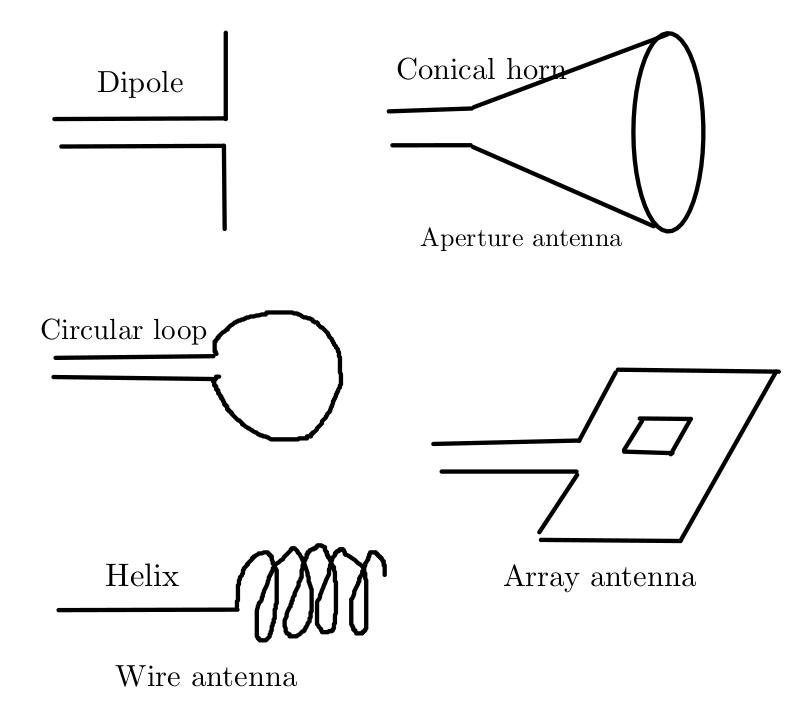
\includegraphics[width=0.3\textwidth]{type.jpg}
			\caption{Some types of antenna}			\label{fig:re6}
\end{figure}

\end{frame}
\begin{frame}{Lý thuyết Antenna}
\begin{itemize}
\item[-] Cơ chế bức xạ
\end{itemize}
\subsubsection{Cơ chế bức xạ}
Xét một đoạn dây dẫn thẳng dài có dòng điện $I$ chạy qua, với $J$ là mật độ dòng $(A/m^2)$, $q_{v}$ là mật độ điện khối $(C/m^3)$ và $v_{d}$ (drift velocity) là tốc độ trôi dạt của điện tích dương, ta cần chứng minh: $J=q_{v}v_{d}$.
\begin{equation*}
\begin{split}
	Q_{total}&=(q_{v}AL) \\
	\Rightarrow I&=\frac{Q_{total}}{t}=\frac{(q_{v}AL)}{L/v_{d}}=q_{v}Av_{d}\\
	\Rightarrow J&=\frac{I}{A}=q_{v}v_{d}
\end{split}
	\end{equation*}
Trong trường hợp dân dẫy có diện tích mặt cắt (cross-section area) cực nhỏ (hay $r\approx 0$) thì ta có thể thay $J$ thành $I$, suy ra:
$$I=q_{v}v_{d}\Rightarrow \frac{dI}{dt}=q_{v}\frac{dv_{d}}{dt}=q_{v}a_{d}$$
Ta viết lại phương trình trên dưới dạng vector:
$$\frac{d\overrightarrow{I}}{dt}=q_{v}\overrightarrow{a_{d}}$$
\end{frame}
\begin{frame}{Lý thuyết Antenna}
Từ phương trình trên ta có thể kết luận:
\begin{enumerate}
	\item Nếu điện tích không chuyển động thì hiện tượng bức xạ không xảy ra. 
	\item Nếu điện tích chuyển động đều thì:
		\begin{itemize}
			\item Trong trường hợp dây dẫn thẳng dài vô hạn, hiện tượng bức xạ không xảy ra.
			\item \alert{Trong trường hợp dây dẫn bị uốn cong, hiện tượng bức xạ \textbf{có xảy ra do vector gia tốc đổi chiều liên tục.} }
		\end{itemize}
	\item Nếu điện tích chuyển động với gia tốc khác $0$ thì hiện tượng bức xạ có xảy ra.
\end{enumerate}
Ta xét một horn antenna được minh họa như sau:
\begin{figure}[h]
			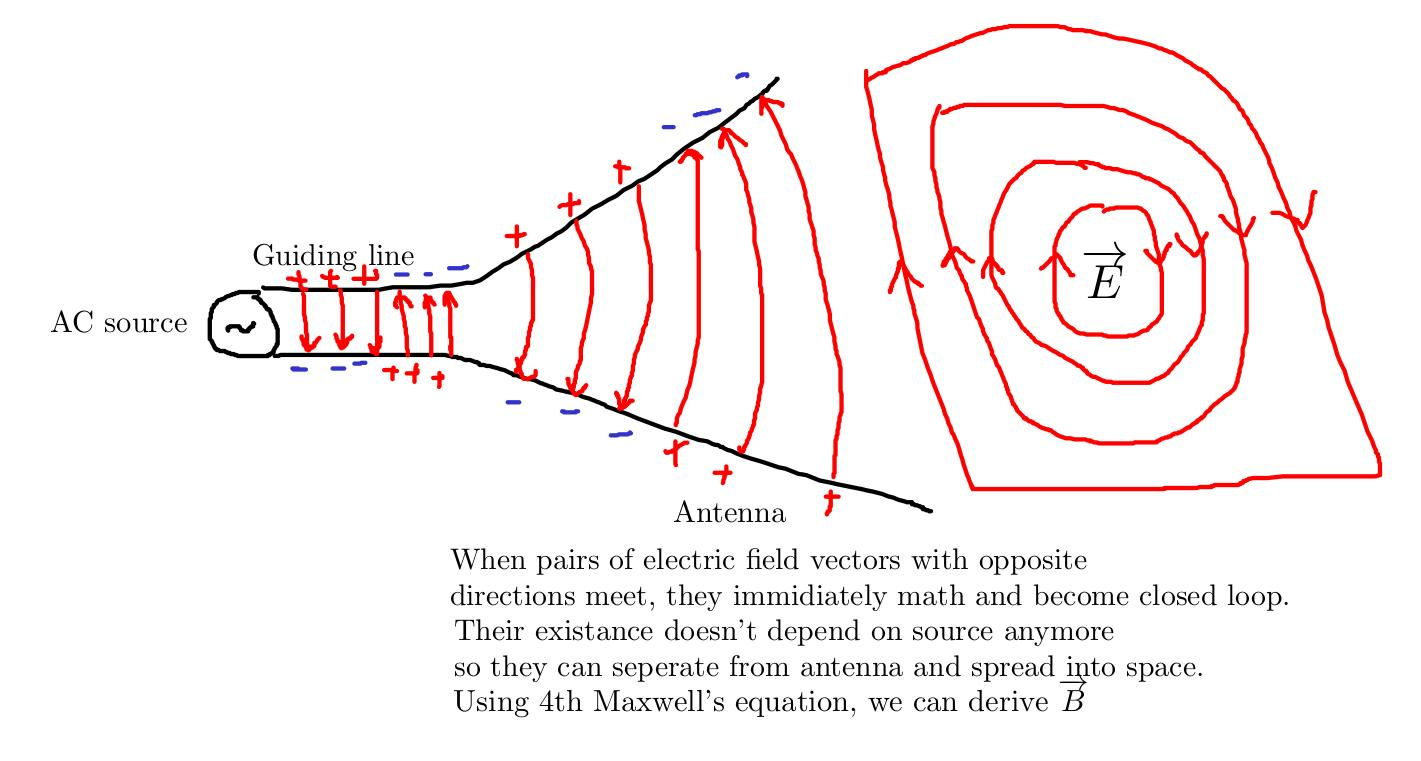
\includegraphics[width=0.9\textwidth]{horn.jpg}
			\caption{Radiation mechanism}			\label{fig:re7}
\end{figure}

\end{frame}
\begin{frame}{Lý thuyết Antenna}
\begin{itemize}
	\item Các tham số cơ bản của Antenna
\end{itemize}
\subsection{Các tham số cơ bản của Antenna}
\begin{itemize}
	\item[-] Giới thiệu các tham số cơ bản
\end{itemize}
\subsubsection{Giới thiệu các tham số cơ bản}
Trước khi phân tích, ta định nghĩa đại lượng $H$ đặc trưng cho cường độ từ trường như sau: $$H=\frac{B}{\mu_{0}}$$
$B$ đặc trưng cho \alert{phân bố của các vector cảm ứng điện từ}, còn $H$ đặc trưng cho \alert{cường độ từ trường}, đây là 2 đại lượng vật lý dễ nhầm và có ý nghĩa hoàn toàn khác nhau.
\\ Ta đổi kí hiệu góc trong phép biến đổi tọa độ cầu (sphere coordinate) từ $(r,\theta,\phi)$ thành $(r,\phi,\theta)$ để hợp với cách quy ước của giáo trình.
\\ Mẫu bức xạ antenna (antenna radiation pattern) được định nghĩa là một hàm số hay đồ thị biểu diễn các tính chất của bức xạ antenna được xác định tại \alert{\textbf{trường xa}} (far-field region). \\Các tính chất tiêu biểu của bức xạ bao gồm công suất, cường độ bức xạ hay độ lớn, hướng, phân cực của trường. Ta sử dụng \alert{\textbf{hệ tọa độ cầu}} để khảo sát các tính chất của bức xạ.
\end{frame}
\begin{frame}{Lý thuyết Antenna}
\begin{figure}[h]
			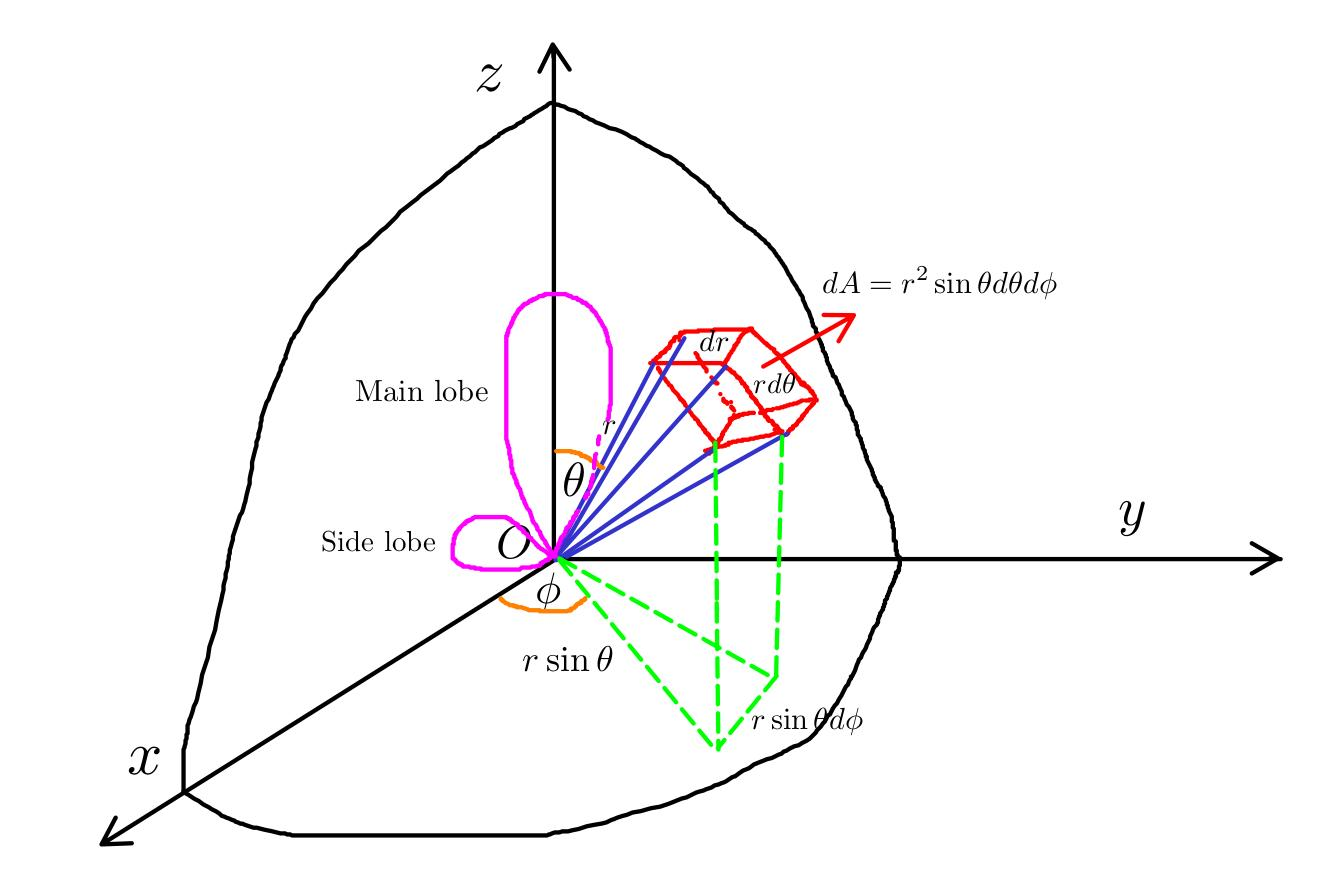
\includegraphics[width=0.9\textwidth]{sphere.jpg}
			\caption{Sphere coordinate to analyze antenna radiation}			\label{fig:re7}
\end{figure}

\end{frame}
\begin{frame}{Lý thuyết Antenna}
\begin{figure}[h]
			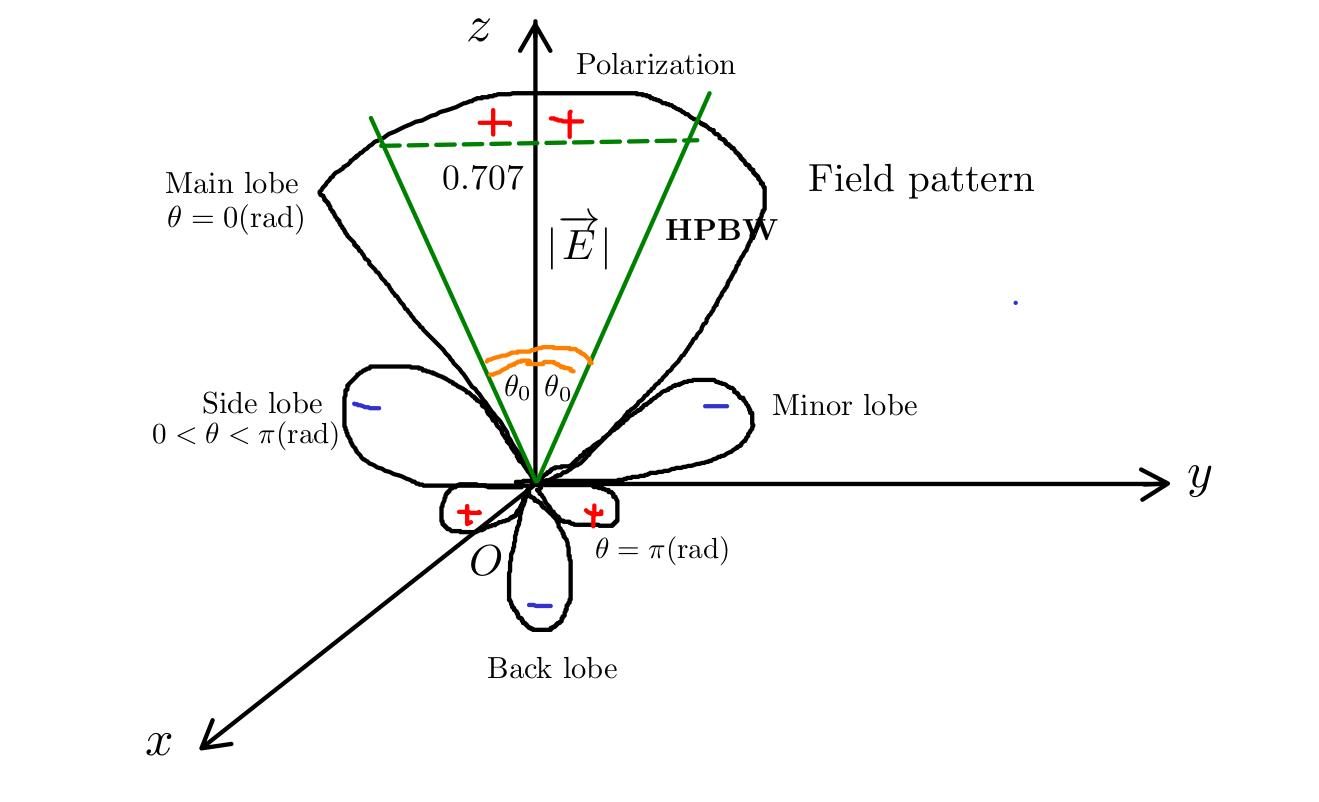
\includegraphics[width=1\textwidth]{linear.jpg}
			\caption{Field pattern (in linear scale)}			\label{fig:re8}
\end{figure}
\end{frame}
\begin{frame}{Lý thuyết Antenna}

\begin{figure}[h]
			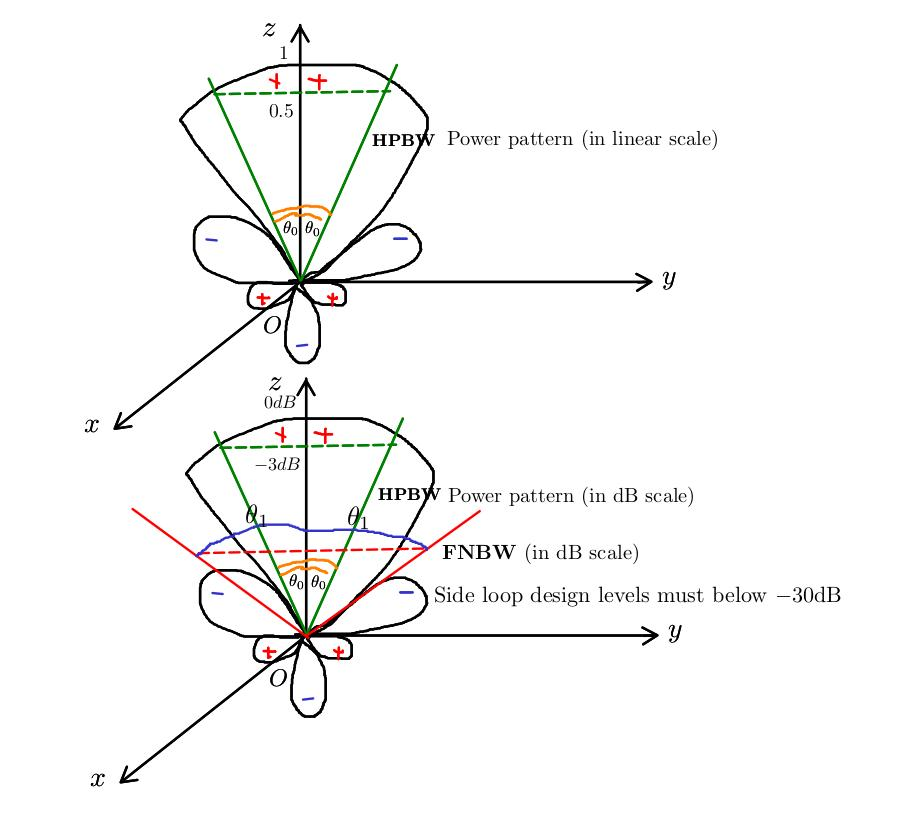
\includegraphics[width=0.8\textwidth]{power.jpg}
			\caption{Power pattern (in dB scale)}			\label{fig:re9}
\end{figure}
\end{frame}
\begin{frame}{Lý thuyết Antenna}
\begin{figure}[h]
			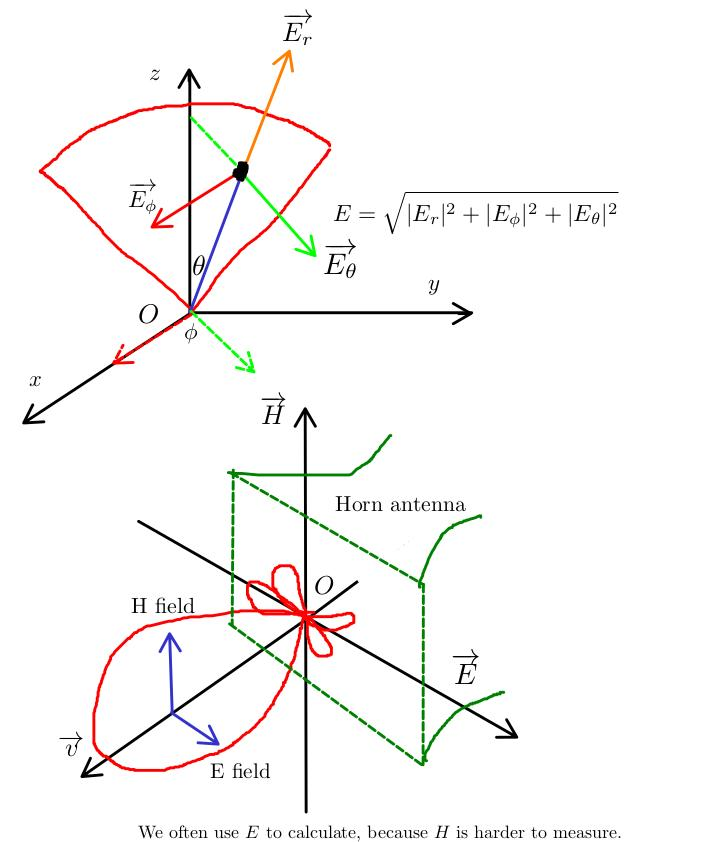
\includegraphics[width=0.61\textwidth]{e.jpg}
			\caption{Principal $E-$ and $H-$ plane patterns}			\label{fig:re10}
\end{figure}

\end{frame}
\begin{frame}{Lý thuyết Antenna}

\begin{figure}[h]
			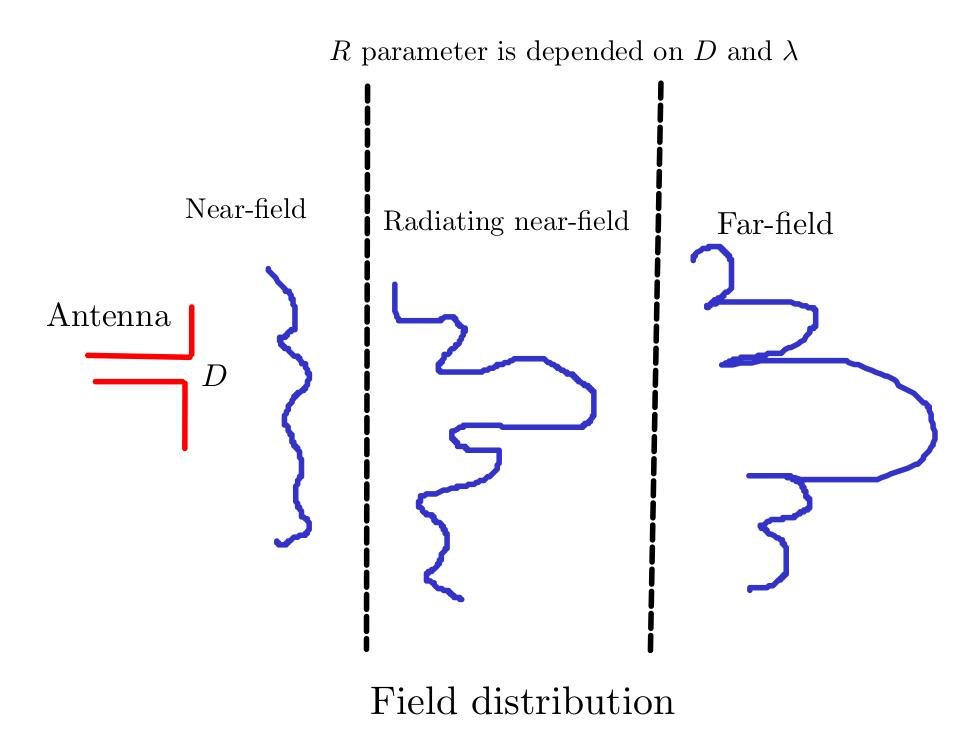
\includegraphics[width=0.8\textwidth]{field.jpg}
			\caption{Types of field}			\label{fig:re10}
\end{figure}
\end{frame}
\begin{frame}{Lý thuyết Antenna}
\begin{figure}[h]
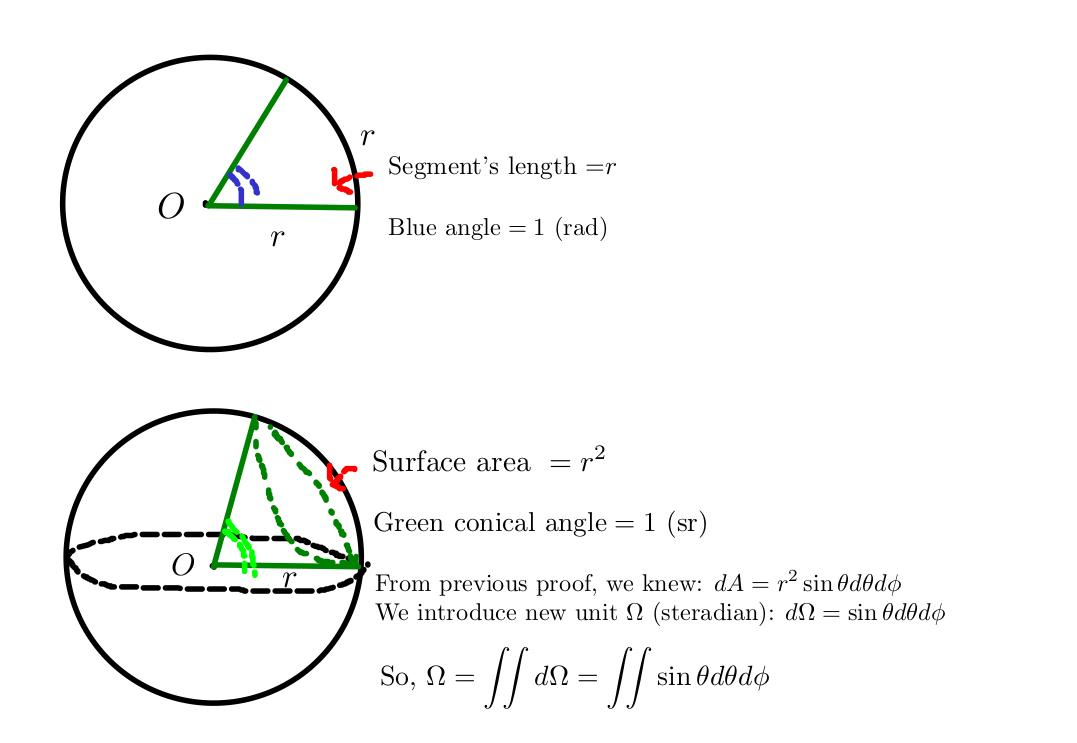
\includegraphics[width=1\textwidth]{sterian.jpg}
\caption{Radian and Sterian}
\end{figure}

\end{frame}
\begin{frame}{Lý thuyết Antenna}
	Ví dụ: hãy tính $\Omega$ (solid angle) của một mặt $S$ kín bị giới hạn bởi: $$S=\{(r,\phi,\theta )|\; 0\leq \phi\leq 2\pi,\;0\leq\theta\leq\frac{\pi}{6}\}$$
	Dễ thấy $$\Omega=\iint\sin{\theta}d\theta d\phi=\int_{0}^{2\pi}\int_{0}^{\frac{\pi}{6}}\sin{\theta}d\theta d\phi=0.8417$$
\begin{itemize}
	\item[-] Công suất bức xạ
\end{itemize}
\subsubsection{Công suất bức xạ}
Từ khái niệm vector Poynting đã được thảo luận ở slide trước, ta định nghĩa kí hiệu mới $\mathscr{W}$ có thứ nguyên $(W/m^2)$ như sau: $$\overrightarrow{\mathscr{W}}=\overrightarrow{\mathscr{E}}\times\overrightarrow{\mathscr{H}}$$
với các kí hiệu viết hoa biểu thị cho \alert{giá trị tức thời}. Vậy ta dễ dàng suy ra độ lớn công suất tức thời trên búp sóng (được biểu diễn bởi mặt S) là: $$\mathscr{P}=\iint_{S}\overrightarrow{\mathscr{W}}\hat n dA=\iint_{S}\overrightarrow{\mathscr{W}}d\overrightarrow{S}$$
với $\hat n$ biểu diễn phương truyền sóng. Ta muốn xây dựng công thức để tìm công suất trung bình (hay công suất bức xạ) $P_{avg}=P_{rad}$ của búp sóng.
\end{frame}
\begin{frame}{Lý thuyết Antenna}
Điện trường hay từ trường của sóng EM lan truyền trong không gian và thời gian, về bản chất là hàm vector có thể được biểu diễn bằng hàm $4$ biến $(x,y,z,t)$:
$$\overrightarrow{E}=\overrightarrow{E(x,y,z)}e^{j\omega t}$$
$$\overrightarrow{H}=\overrightarrow{H(x,y,z)}e^{j\omega t}$$
Ta định nghĩa độ lớn tức thời của các giá trị cường độ điện trường và từ trường:
$$\overrightarrow{\mathscr{E}}=\Re{(\overrightarrow{E})}$$
$$\overrightarrow{\mathscr{H}}=\Re{(\overrightarrow{H})}$$
Biến đổi một chút, ta thu được:
\begin{equation*}
\begin{split}
	{\overrightarrow{\mathscr{H}}}=\frac{1}{2}\Re{(\overrightarrow{H}+\overrightarrow{H^*})}
	\Rightarrow \overrightarrow{\mathscr{W}}=\frac{1}{2}\Re{(\overrightarrow{E}\times\overrightarrow{H})}+\frac{1}{2}\Re{(\overrightarrow{E}\times\overrightarrow{H^*})}
\end{split}
\end{equation*}
Giữ lại thành phần không phụ thuộc vào biến thời gian, ta thu được $W_{avg}$:
$$\overrightarrow{W_{avg}}=\frac{1}{2}\Re{(\overrightarrow{E}\times\overrightarrow{H^*})}$$
Dùng định nghĩa tích phân mặt, ta có:
$$P_{avg}=P_{rad}=\iint_{S}\overrightarrow{W_{avg}}d\overrightarrow{S}=\alert{\iint_{S}\frac{1}{2}\Re{(\overrightarrow{E}\times\overrightarrow{H^*})}dS}$$
\end{frame}
\begin{frame}{Lý thuyết Antenna}
Ví dụ: tính công suất bức xạ trung bình của một bức xạ lý tưởng đẳng hướng (bức xạ đều ra tất cả các hướng với độ lớn vector Poyting là hằng số).
\begin{equation*}
\begin{split}
	P_{avg}&=\iint_{S}W_{0}\hat n_{r} dA=\iint_{S}(W_{0}\hat n_{r}) \hat n_{r}r^2\sin{\theta}d\theta d\phi=\int_{0}^{2\pi}\int_{0}^{\pi}W_{0}r^2\sin{\theta}d\theta d\phi \\
	       &=4\pi W_{0}r^2
\end{split}
\end{equation*}
\begin{itemize}
	\item[-] Cường độ bức xạ
\end{itemize}
\subsubsection{Cường độ bức xạ}
Cường độ bức xạ $U$ là đại lượng vô hướng, được định nghĩa là công suất bức xạ từ antenna trên một đơn vị solid angle. $$U=r^2W_{rad}$$ Ta suy ra công thức tìm $P_{rad}$ khác:
$$P_{rad}=\iint_{\Omega}Ud\Omega=\iint_{\Omega}U\sin{\theta}d\theta d\phi$$
với công thức tìm vi phân solid angle theo steradian đã được chứng minh ở trên.
\\ Ví dụ: tính cường độ bức xạ $U_{0}$ của một nguồn bức xạ đẳng hướng có công suất trung bình $P_{rad}$.
 \begin{equation*}
\begin{split}
	P_{rad}=\iint_{\Omega}U_{0}d\Omega=\iint_{\Omega}U_{0}\sin{\theta}d\theta d\phi=U_{0}\int_{0}^{2\pi}\int_{0}^{\pi}\sin{\theta}d\theta d\phi \Rightarrow U_{0}=\frac{P_{rad}}{4\pi}
\end{split}
\end{equation*}

\end{frame}

\begin{frame}{Hướng nghiên cứu tiếp theo}
Học nốt chapter 2 + 3 của textbook Antenna Theory.
\section{Hướng nghiên cứu tiếp theo}
\end{frame}
\end{document}

